\documentclass[article,shortnames]{jss}
%%%%%%%%%%%%%%%%%%%%%%%%%%%%%%
%% declarations for jss.cls %%%%%%%%%%%%%%%%%%%%%%%%%%%%%%%%%%%%%%%%%%
%%%%%%%%%%%%%%%%%%%%%%%%%%%%%%

%% almost as usual
\author{Stefan R\"odiger\\L.U.A.S. & Charit\'e
	\And Prasenjit Kapat\\Plus Affiliation
	\And Meik Michalke\\Plus Affiliation
	\And Thomas Friedrichsmeier\\Ruhr-University Bochum}
\title{RKWard - A Comprehensive Graphical User Interface and Integrated Development Environment for Statistical Analysis With {R}}

%% for pretty printing and a nice hypersummary also set:
\Plainauthor{Stefan R\"odiger, Prasenjit Kapat, Meik Michalke, Thomas Friedrichsmeier} %% comma-separated
\Plaintitle{RKWard - A Comprehensive Graphical User Interface and Integrated Development Environment for Statistical Analysis With R} %% without formatting
\Shorttitle{RKWard a GUI to {R}} %% a short title (if necessary)

%% an abstract and keywords
\Abstract{
  R is a free, open-source implementation of the S statistical computing
language and programming environment. The current status of R is a
command line driven interface with no advanced standard Graphical User
Interface (GUI) but it includes tools for building such. Over the past
years proprietary and non-proprietary GUI solutions, based on internal
or external tool kits, with different scopes and technological concepts
have emerged. In this paper we discuss RKWard which aims to be both a
comprehensive cross-platform GUI and Integrated Development Environment
(IDE) for R. RKWard is based on the KDE software libraries. Statistical
procedures and plots are implemented using an extendable plugin
architecture based on ECMA script (JavaScript), R, and XML. RKWard
provides an excellent tool to manage different types of data objects;
even allowing for seamless editing of certain types. The objective of
RKWard is to provide a portable and extensible R interface for both
basic and advanced statistical and graphical analysis while not
compromising on flexibility and modularity of the R programming
environment itself.
}
\Keywords{GUI, IDE, R, plugin, cross-platform}
\Plainkeywords{keywords, comma-separated, not capitalized, Java} %% without formatting
%% at least one keyword must be supplied

%% publication information
%% NOTE: Typically, this can be left commented and will be filled out by the technical editor
%% \Volume{13}
%% \Issue{9}
%% \Month{September}
%% \Year{2004}
%% \Submitdate{2004-09-29}
%% \Acceptdate{2004-09-29}

%% The address of (at least) one author should be given
%% in the following format:
\Address{
  Stefan R\"odiger\\
  Lausitz University of Applied Sciences (L.U.A.S)\\
  Department of Bio-, Chemistry and Process Engineering\\
  AND\\
  Center for Cardiovascular Research (CCR)\\
  Charit\'e, Germany\\
  E-mail: \email{stefan\_roediger@gmx.de}
}

%% NOTE: It appears only the last entered address is actually used. So I guess we should only give Stefan's (the corresponding author).
% \Address{
%  Prasenjit Kapat\\
%  Affiliation\\
%  Department\\
%  E-mail: \email{noname@here.org}
% }
% \Address{
%  Meik Michalke\\
%  Affiliation\\
%  Department\\
% }
% \Address{
%  Thomas Friedrichsmeier\\
%  Affiliation\\
%  Department\\
%  E-mail: \email{noname@here.org}
% }

%% It is also possible to add a telephone and fax number
%% before the e-mail in the following format:
%% Telephone: +43/1/31336-5053
%% Fax: +43/1/31336-734

%% for those who use Sweave please include the following line (with % symbols):
%% need no \usepackage{Sweave.sty}

%% end of declarations %%%%%%%%%%%%%%%%%%%%%%%%%%%%%%%%%%%%%%%%%%%%%%%


\begin{document}

%% include your article here, just as usual
%% Note that you should use the \pkg{}, \proglang{} and \code{} commands.

%% For the time being, each main chapter is in a separate file, so we can
%% work in parallel, easier
% !TEX root = RKWard_paper.tex
\section{Background and motivation}
\label{background}
In mid 1993 Ihaka and Gentleman published initial efforts on the computing
language and programming environment \proglang{R} on the \emph{s-news} mailing list. Ambitions for
this project were to develop an \proglang{S}-like language without inheriting memory
and performance issues. The source code of \proglang{R} was finally released in 1995, and 
since 1997 development has evolved under the umbrella of the \proglang{R} 
Development Core Team \citep{RDCT2001, RDCT2010, Ihaka_Gentlemen_1993}.
\proglang{R} does not include an advanced cross-platform graphical user interface (GUI) as known from other
statistical software packages. However, \proglang{R} includes tools for building GUIs
mainly based on \proglang{Tlc/Tk} \citep{Dalgaard2001, Dalgaard2002}. Meanwhile a
plethora of \proglang{R} GUIs have emerged (see \url{http://www.sciviews.org/_rgui/} for a
comprehensive list). In 2005 John Fox released version 1.0 of \proglang{R} Commander (package \pkg{Rcmdr}), which
can be considered a milestone in \proglang{R} GUI development; it was the first GUI
implementation that was able to make statistical tests,
plots and data manipulation easily accessible for \proglang{R} novices.
John Fox stated that \pkg{Rcmdr}'s target was to provide
functionality for basic-statistical courses, though the features have increased over
time beyond this \citep{Fox2005, Fox2007}. In November 2002 Thomas Friedrichsmeier
started the \pkg{RKWard} open-source software project with the goal to create a GUI for
\proglang{R} based on \pkg{KDE}\footnote{\url{http://www.kde.org/}} and \pkg{Qt}\footnote{\url{http://qt.nokia.com/}} technologies.

The scope of \pkg{RKWard} is deliberately broad, targeting both \proglang{R} novices and experts.
For the first group, the aim is to allow any person with knowledge on
statistical procedures to start using \pkg{RKWard} for their everyday work 
without having to learn anything about the \proglang{R} programming language,
at least initially. At the same time, \pkg{RKWard} tries to support users who want to learn and
exploit the full flexibility of the \proglang{R} language for automating or customizing
an analysis. At the other end of the learning curve, \pkg{RKWard} provides advanced integrated development environment (IDE)
features to \proglang{R} experts to assist in writing \proglang{R} scripts. Yet, the idea
is that \proglang{R} experts too will benefit from the availability of task-oriented GUI
dialogs, such as when exploring an unfamiliar type of analysis
or by allowing to implement routinely performed tasks as a GUI element. In
addition, many features like the integrated data editor and the plot preview 
will be useful to \proglang{R} novices and \proglang{R} experts alike in their everyday work
(see Section~\ref{sec:user_interface}).

\pkg{RKWard} provides a high level of transparency about the steps that are needed to
perform any supported task in \proglang{R}, in order to make it easy for the user to see
complete codes for all GUI actions\footnote{
  This distinguishes \pkg{RKWard} from \proglang{R} GUIs such as \pkg{Red-R} (\url{http://www.red-r.org/}), which 
  specifically aims to hide the complexities of the \proglang{R} programming language, following the concept of visual data-flow 
  programming \citep{Sutherland1966}. In contrast, \pkg{RKWard} limits itself to generate \proglang{R} code from GUI settings.
}. In doing so, \pkg{RKWard} deliberately generates
comparatively verbose code. It avoids wrapping complex sequences of data
manipulation or analysis into custom high-level \proglang{R} functions. The task of
providing high-level functions is logically independent of the development of the
GUI frontend, and should best be addressed in dedicated \proglang{R} packages, where necessary.
This approach allows to make better use of the modular design of \proglang{R}, avoids
locking-in users to a specific GUI application, and provides them with more options for
customizing the generated code patterns.

While \pkg{RKWard} tries to address users wishing to learn \proglang{R}, it is specifically not
designed as a teaching tool (such as \pkg{Rcmdr} or \pkg{TeachingDemos}), but as
a productive tool. Dialogs for statistical procedures in \pkg{RKWard} do not
necessarily show a one-to-one correspondence to the underlying steps in \proglang{R}, but are
rather oriented at statistical tasks. Furthermore, \pkg{RKWard} does not impose
artificial limitations on how users can work with the application. For example,
the user is not limited to using only one \code{data.frame} or one model at a
time. \pkg{RKWard} is designed to allow users to create custom GUI dialogs
easily (see Sections~\ref{sec:technical_plugins} and \ref{sec:example_plugin}).

\pkg{RKWard} is licensed under the terms of the GNU General Public License Version 2
or higher. However, due to its dependencies, \pkg{RKWard} binaries are effectively
distributable only under the terms of Version 2 of the license. Parts of the documentation are available under the
GNU Free Documentation License. While the project remains in constant development, a growing
number of users employs \pkg{RKWard} in productive scenarios. The source code,
selected binaries and documentation is hosted at SourceForge
(\url{http://rkward.sourceforge.net/}). Selected key milestones of the development of \pkg{RKWard} are
visualized in Figure~\ref{fig:timeline}.

\begin{figure}[t!]
 \centering
 \includegraphics[clip=true,trim=0cm 5.7cm 0cm 5.7cm,width=16cm]{../figures/timeline.pdf}
 \caption{Timeline of important development milestones and changes in \pkg{RKWard}.
          Time is presented on an arbitrary scale. Here \pkg{Qt}3 and \pkg{Qt}4 refers to the 3.x and
          4.x versions of the \pkg{Qt} libraries, respectively and \pkg{KDE}4 refers to the
          4.x version of the \pkg{KDE} libraries.}
 \label{fig:timeline}
\end{figure}

In this paper we will first give an overview over the main GUI elements and
features of \pkg{RKWard} (Section~\ref{sec:user_interface}), followed by a short example 
of a simple \pkg{RKWard} session (Section~\ref{sec:using_RKWard}). Next, technical 
details of the implementation will be discussed, comparing them briefly to 
competing GUI solutions, where appropriate (Section~\ref{sec:technical}).
Finally, we show an example for creating a plugin extension to \pkg{RKWard} 
(Section~\ref{sec:example_plugin}).

%%\include{usage}
%!TEX root=RKWard_paper.tex
\section{Technical design}
\label{sec:technical}
In this section we will give a compact overview of the key aspects of RKWard's
technical design. We will give slightly more attention to the details of the
plugin framework (Section~\ref{sec:technical_plugins}) used in RKWard, since this is central to the extensibility of
RKWard.

\subsection{Asynchronous command execution}
\label{sec:technical_asynchronous}
One central design decision in the implementation of RKWard is that the
interface to the \proglang{R} engine operates asynchronously. The intention is to
keep the application usable to a high degree, even during the computation of
time-consuming analysis. For instance, while waiting for the estimation of a
complex model to complete, the user should be able to continue to use the GUI to
prepare the next analysis. Asynchronous command execution is also a prerequisite
for an implementation of the plot-preview feature (see Section~\ref{sec:plot_previews}). Commands
generated from plugins or user actions are placed in queue and are evaluated in
a separate thread in the order they were submitted\footnote{
    It is possible, and in some cases necessary, to enforce a different order of command execution in
    internal code. For instance, RKWard makes sure that no user command can
    potentially interfere while RKWard is loading the data of a \code{data.frame} for
    editing.
}. The asynchronous design implies that RKWard avoids relying on the
\proglang{R} engine during interactive use. This is one of several reasons for
the use of \proglang{ECMAScript} in plugins, instead of scripting using
\proglang{R} itself (see Sections~\ref{sec:technical_toolkit} and \ref{sec:technical_plugins}).
A further implication is that RKWard avoids querying information about the
existence and properties of objects in \proglang{R} interactively. Rather,
RKWard keeps a representation of \proglang{R} objects and their basic properties
(e.\,g., class and dimensions), which is used for the workspace browser (Section~\ref{sec:workspace_browser_object_viewer}),
object name completion, function argument hinting, and
other places. The object representation includes objects in all environments
in the search path, and any objects contained within these environments in a
hierarchical tree\footnote{
    Currently, environments of functions or formulas are not taken into account.
}. The representation of \proglang{R} objects is gathered
pro-actively. This has a notable impact on performance when loading packages.
Specifically, objects which would usually be ``lazy loaded'' only when needed \citep[see][]{Ripley2004} are
accessed in order to fetch information on their properties. This means the data
has to be loaded from disk; however, the memory is freed immediately after fetching
information on the object. Additionally, for packages with extremely large number of objects, RKWard
provides an option to exclude specific packages from scanning the object structures.

A further side-effect of the asynchronous threaded design is that there is
inherently a rather clear separation between the GUI code and the code making direct use
of the \proglang{R} application programming interface (API) (see also Figure~\ref{fig:design_sketch}). 
In the current development version, the evaluation
of \proglang{R} commands has even been moved into a separate process. Therefore in future releases it could 
be made possible to run GUI and \proglang{R} engine on different computers.

\begin{figure}[t!]
 \centering
 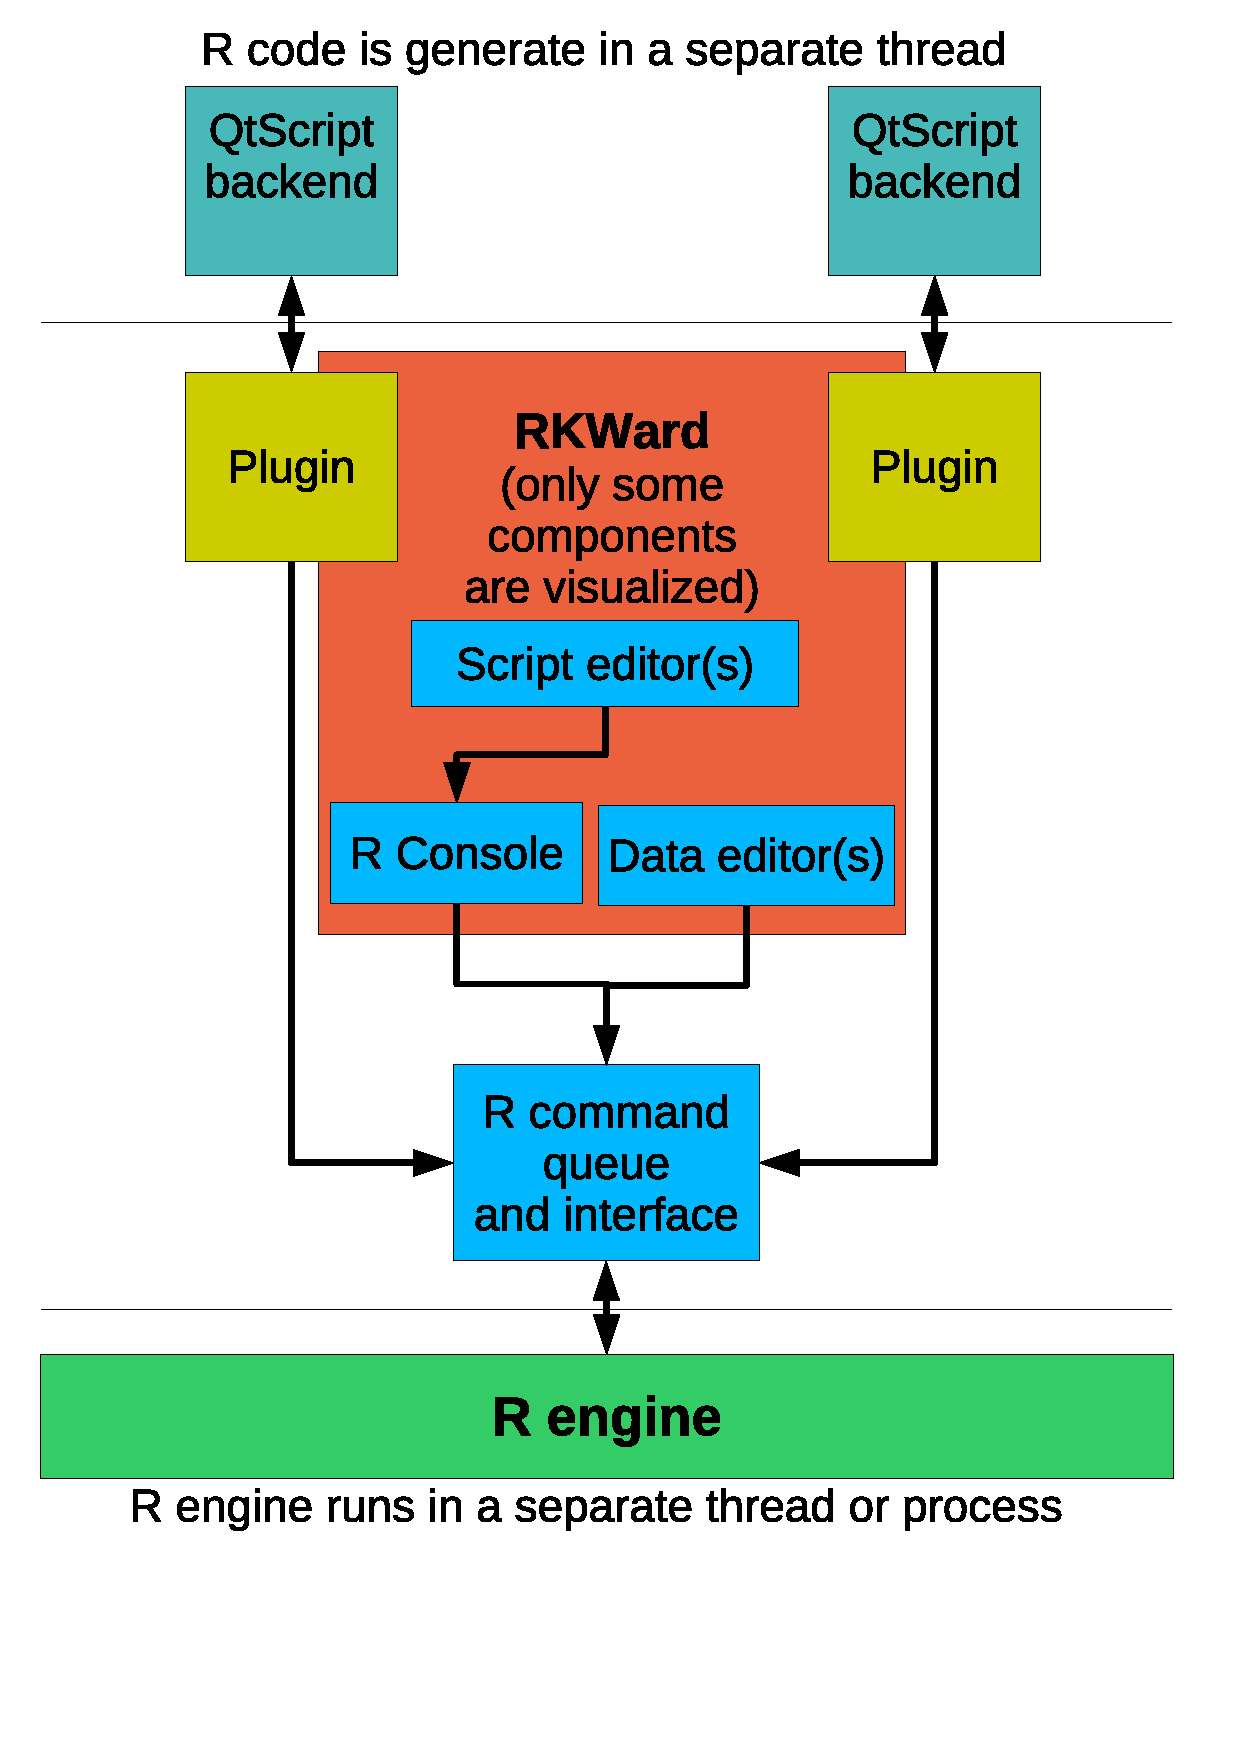
\includegraphics{../figures/design_sketch.pdf}
 \caption{Technical design of RKWard. Only a few central components are visualized.
 All communication with the \proglang{R} engine is passed through a single interface living in the main application thread. The \proglang{R} engine itself
 runs in a separate thread (or in a separate process). 
 Separate threads are also used to generate \proglang{R} code from plugins.
}
 \label{fig:design_sketch}
\end{figure}

\subsection{Object modification detection}
\label{sec:technical_omd}
RKWard allows the user to run arbitrary commands in \proglang{R} at any time, even while
editing a \code{data.frame} or while selecting objects for analysis in a GUI dialog. Any user
command can potentially add, modify, or remove objects in \proglang{R}. RKWard tries to
detect such changes in order to always display accurate information in the
workspace browser, object selection lists, and object views. Beyond that,
detecting any changes is particularly important with respect to objects which
are currently being edited in the data editor (which provides an illusion
of in-place editing, see Section~\ref{sec:spreadsheet}). Here, it is necessary to synchronize
the data between \proglang{R} and the GUI in both directions.

For simplicity and performance, object modification detection is only
implemented for objects inside the ``global environment'' (including environments
inside the global environment), since this is where changes are typically done.
Currently, object modification detection is based on active bindings.
Essentially, any object which is created in the global environment is first
moved to a hidden storage environment, and then replaced with an active binding.
The active binding acts as a transparent proxy to the object in the storage
environment, which registers any write-access to the object\footnote{
    This is similar to the approach taken in the \pkg{trackObjs} package \citep{Plate2009}.
}.

The use of active bindings has significant performance implications when
objects are accessed very frequently. This is particularly notable where an
object inside the global environment is used as the index variable in a loop,
as illustrated by the following example. When control returns to the top level
prompt, after the first assignment, \code{i} will become subject to object modification
detection (i.\,e., it will be wrapped into an active
binding). The subsequent \code{for} loop will then run slow.

\begin{Code}
R> i <- 1
R> for (i in 1:100000) i + i
\end{Code}

In contrast, in the following example, \code{i} is a local object, and will not
be replaced by an active binding. Therefore the loop will run approximately as fast
as in a plain \proglang{R} session:

\begin{Code}
R> f <- function () {
R+    i <- 1
R+    for (i in 1:100000) i + i
R+ }
R> f ()
\end{Code}

Future versions of RKWard will try to avoid this performance problem. 
One approach that is currently under consideration is to simply perform
a pointer comparison of the SEXP records of objects in global environment with
their copies in a hidden storage environment. Due to the implicit sharing of
SEXP records \citep{RDCT2010a, RDCT2010b}, this should provide for a reliable
way to detect changes for most types of \proglang{R} objects, with comparatively low memory
and performance overhead. Special handling will be needed for environments and
active bindings.

\subsection{Choice of toolkit and implementation languages}
\label{sec:technical_toolkit}
In addition to \proglang{R}, RKWard is based on the \proglang{KDE} libraries, which are in turn based
on \proglang{Qt}, and implemented mostly in \proglang{C++}. Compared to many competing libraries,
this constitutes a rather heavy dependency. Moreover, the \proglang{KDE} libraries are
still known to have portability issues especially on Mac OS X, and to some degree
also on the Windows platform.

The major reason for choosing the \proglang{KDE} and \proglang{Qt} libraries was their 
many high level features which have allowed RKWard development to make quick
progress despite limited resources. Most importantly, the \proglang{KDE} libraries provide a
full featured text editor \citep{CullmannND} as a component which can be
seamlessly integrated into a host application using the KParts technology
\citep{Faure2000}. Additionally, another KPart provides \proglang{HTML} browsing capabilities in a
similarly integrated way. The availability of KWord \citep{KWord} as an
embeddable KPart might prove useful in future versions of RKWard, when better
integration with office suites will be sought.

Another technology from the \proglang{KDE} libraries that is important to the development
of RKWard is the ``XMLGUI'' technology
\citep{Faure2000}. This is especially helpful in providing an integrated GUI across
the many different kinds of document windows and tool views supported in RKWard.

Plugins in RKWard rely on \proglang{XML} (extensible markup language)\footnote{\url{http://www.w3.org/XML/}}
and \proglang{ECMAScript}\footnote{\url{http://www.ecmascript.org/}} (see Section~\ref{sec:technical_plugins}). \proglang{XML} is not
only well suited to describe the layout of the GUI of plugins, but simple
functional logic can also be represented \citep[see also][]{Visne2009}. \proglang{ECMAScript} was
chosen for the generation of \proglang{R} commands within plugins, in particular due to its
availability as an embedded scripting engine inside the \proglang{Qt} libraries. While at
first glance \proglang{R} itself would appear as a natural choice of scripting language as
well, this would make it impossible to use plugins in an asynchronous way.
Further, the main functional requirement in this place is the manipulation and
concatenation of text strings. While \proglang{R} provides support for this, concatenating
strings with the \code{+}-operator, as available in \proglang{ECMAScript}, allows for a much
more readable way to perform such basic text manipulation.

\subsection{On-screen graphics windows}
\label{sec:technical_graphics}
Contrary to the approach used in \pkg{JGR} \citep{JGR2010}, RKWard does
not technically provide a custom on-screen graphics device. RKWard detects when
new graphics windows are created via calls to \code{X11()} or \code{windows()}. These windows
are then ``captured'' in a platform dependent way (based on the XEmbed \citep{Ettrich2002} protocol
for X11, on reparenting for the Windows platform). An RKWard menu bar and a
toolbar is then added to these windows to provide added functionality. While
this approach requires some platform dependent code, any corrections or
improvements made to the underlying \proglang{R} native devices will automatically be
available in RKWard.

A recent addition to the on-screen device is the ``plot history'' feature which
adds a browsable list of plots to the device window. Since RKWard does not use a
custom on-screen graphics device, this feature is implemented in a package
dependent way. For example, as of this writing, plotting calls that use either
the ``standard graphics system'' or the ``\pkg{lattice} system'' can be added to the plot
history; other plots are drawn but not added. The basic procedure is to identify
changes to the on-screen canvas and record the existing plot before a new plot
wipes it out. A single global history for the recorded plots is maintained
which is used by all the on-screen device windows. This is similar to the
implementation in \proglang{Rgui.exe} (Windows), but unlike the one in \proglang{Rgui.app} 
(Mac OS X). Each such device window points to a position in the history
and behaves independently when recording a new plot or deleting an existing
one.

The \pkg{lattice} system is implemented by inserting a hook in the \code{print.lattice()}
function. This hook retrieves and stores the \code{lattice.status} object from the
\code{lattice:::.LatticeEnv} environment, thereby making \code{update()} calls on trellis
objects transparent to the user. Any recorded trellis object is then replayed
using \code{plot.lattice()}, bypassing the recording mechanism. The standard graphics
system, on the other hand, is implemented differently because the hook in
\code{plot.new()} is ineffective for this purpose. A customized function is overloaded
on \code{plot.new()} which stores and retrieves the existing plot, essentially, using
\code{recordPlot()} and replays them using \code{replayPlot()}.

The actual plotting calls are tracked using appropriate \code{sys.call()} commands in
the hooks. These call strings are displayed as a drop-down menu on the toolbar
for non-sequential browsing (see Figure~\ref{fig:plot_history}) providing a very intuitive browsing
interface unlike the native implementations in \code{windows()} and \code{quartz()} devices.

\subsection{Plugin infrastructure}
\label{sec:technical_plugins}
One of the earliest features of RKWard was the extensibility by plugins.
Basically, plugins in RKWard provide complete GUI-dialogs, or re-usable
GUI-components, which accept user settings and translate those user settings
into \proglang{R} code\footnote{
    Plugins are also used in some other contexts within RKWard, for instance, the
    integrated text editor (kate part) supports extensions via plugins and user scripts. At this point we
    will focus only on plugins generating \proglang{R} code.
}. Thus, the plugin framework is basically a tool set used to define
GUIs for the automatic generation of \proglang{R} code.

Much of the functionality in RKWard is currently implemented as plugins. For example, importing different file
formats relying on the \pkg{foreign} package is achieved by this approach. Similarly,
RKWard provides a modest GUI driven tool set for statistical analysis,
especially for item response theory (IRT), distributions, and descriptive
statistical analysis.

\subsubsection{Defining a plugin}
\label{sec:technical_plugins_defining}
Plugins consist of four parts as visualized in Figure~\ref{fig:plugin_structure} 
\citep[see Section~\ref{sec:example_plugin} for an example; for a complete
manual, see][]{Friedrichsmeier2010}:

\begin{figure}[b!]
 \centering
 \includegraphics[width=8cm]{../figures/plugin_structure.pdf}
 \caption{Plugin structure of RKWard. One or more plugins are declared in a ``plugin map''. Each plugin is defined by
 two \proglang{XML} files, and one \proglang{ECMAScript} file.}
 \label{fig:plugin_structure}
\end{figure}

\begin{itemize}
    \item
    An \proglang{XML} file (Section~\ref{sec:defining_menu_hierarchy}), 
    called a ``plugin map'', is used to declare one or more plugins, each
    with a unique identifier. For most plugins, the plugin map also defines the
    placement in the menu hierarchy. Plugin maps are meant to represent groups of
    plugins. Users can disable/enable such groups of plugins in order to reduce the
    complexity of the menu hierarchy.

    \item
    A second \proglang{XML} file describes the plugin GUI layout itself (Section~\ref{sec:defining_dialog_ui}). 
    Most importantly this includes
    the definition of the GUI-layout and GUI-behavior. High level GUI-elements can
    be defined with simple \proglang{XML}-tags. Layout is based on ``rows'' and ``columns'',
    instead of pixel counts. In most cases this allows for a very sensible resizing
    behavior. RKWard supports single-page dialogs and multi-page wizards, however,
    most plugins define only a single-page GUI. GUI behavior can be programmed by
    connecting ``properties'' of the GUI elements to each other. For example, the state
    of a checkbox could be connected to the ``enabled'' property of a dependent
    control. More complex logic is also supported, as is procedural scripting of GUI
    behavior using \proglang{ECMAScript}.

    \item
    A separate \proglang{ECMAScript} file (Section~\ref{sec:generating_r_code_from_ui_settings}) 
    is used to translate GUI settings into \proglang{R}
    code\footnote{
        In earlier versions of RKWard, \proglang{PHP} was used
        as a scripting engine, and \proglang{PHP} interpreters were run as separate processes.
        Usage of \proglang{PHP} was abandoned in RKWard version 0.5.3 for reasons of performance and simplicity.
    }. This \proglang{ECMAScript} file is evaluated asynchronously in a separate thread. RKWard
    currently enforces structuring the code into three separate sections for
    preprocessing, calculating, and printing results. The generated code is always
    run in a local environment, in order to allow the use of temporary variables
    without the danger of overwriting user data.

    \item
    A third \proglang{XML} file defines a help page. This help page usually links to the \proglang{R} help
    pages of the main functions/concepts used by the plugin, as well as to other 
    related RKWard help pages. Compared to \proglang{R} help
    pages, the plugin help pages try to give more hands-on advice on using the
    plugin. Plugins can be invoked from their help page by clicking on a link near
    the top, which can be useful after following a link from a related help page.
\end{itemize}

Changes to the source code of these elements take effect without the requirement to recompile RKWard.

\subsubsection{Embedding and reuse of plugins}
\label{sec:technical_plugins_embedding}
RKWard supports several mechanisms for modularization and re-use of
functionality in plugins. File inclusion is one very simple but effective
mechanism, which can be used in the \proglang{ECMAScript} files, but is also supported in
the \proglang{XML} files. In script files, this is most useful by defining common functions
in an included file. For the \proglang{XML} files, the equivalent is to define ``snippets''
in the included file, which can then be inserted.

A third mechanism allows to completely embed one plugin into another. For
instance the \code{plot\_options} plugin is used by many plugins in RKWard, to provide
common plot options such as labels, axis options, and grids. Other plugins
can embed it using the \code{embed}-tag in their \proglang{XML} file (the plugin supports
hiding irrelevant options). The generated code portions can be fetched from the
\proglang{ECMAScript} file just like any other GUI settings, and inserted into the complete
code. Other examples of embedded plugins are options for histograms, barplots,
and empirical cumulative distribution function (ECDF) plots (which in turn embed the generic plot options plugin).

\subsubsection{Enforcing a consistent interface}
\label{sec:technical_plugins_consistency}
RKWard tries to make it easy to create a consistent interface in all plugins.
GUI-wise this is supported by providing high-level GUI elements, and embeddable
clients. Also, the standard elements of each dialog (``Submit'', and
``Cancel'' buttons, on-the-fly code view, etc.) are hard coded. Up to version
0.5.3 of RKWard it was not possible to use any GUI elements in plugins which
were not explicitly defined for this purpose. In the current development
version, theoretically, all GUI elements available from \proglang{Qt} can be inserted,
where necessary.

For generating output, the function \code{rk.header()} can be used to print a
standardized caption for each piece of output. Printing results in vector or
tabular form is facilitated by \code{rk.results()}. A wide range of objects can be
printed using \code{rk.print()}, which is just a thin wrapper around the
\code{HTML()} function of the \pkg{R2HTML} package \citep{Lecoutre2003} in the current
implementation. The use of custom formatting with \proglang{HTML} is possible, but
discouraged. Standard elements such as a horizontal separator, and the ``Run again''
link (see Section~\ref{sec:results_output}) are inserted automatically, without the need to define
them for each plugin.

Regarding the style of the generated \proglang{R} code, enforcing consistency is harder,
but plugins which are to become part of the official RKWard application are
reviewed for adherence to some guidelines. Perhaps the most important guidelines
are 

\begin{itemize}
  \item 
  Write readable code, which is properly indented, and commented where necessary.

  \item 
  Do not hide any relevant computations from the user by performing them in the
  \proglang{ECMAScript}. Rather, generate \proglang{R} code which will perform
  those computations, transparently.

  \item
  Plugins can be restricted to accept only certain types of data (such as only one-dimensional numeric data).
  Use such restrictions where appropriate to avoid errors, but be very careful not to add
  too many of them.
\end{itemize}

\subsubsection[Handling of R package dependencies]{Handling of \proglang{R} package dependencies}
\label{sec:technical_plugins_dependencies}
A wide range of plugins for diverse functionality is present in RKWard,
including plots (e.\,g., boxplot) or standard tests (e.\,g., Student's t-test)\footnote{
  At the time of this writing, there are 164 user-accessible plugins in RKWard.
  Listing all is beyond the scope of this article.
}. Some
of the plugins depend on \proglang{R} packages other than the recommended \proglang{R} base packages.
Examples herein are the calculation of kurtosis, skewness or the exact Wilcoxon
test.

RKWard avoids loading all these packages pro-actively, as \pkg{Rcmdr} does. Rather,
plugins which depend on a certain package simply include an appropriate call to
\code{require()} in the pre-processing section of the generated \proglang{R} code. The \code{require()}
function is overloaded in RKWard, in order to bring up the package-installation
dialog (see Section~\ref{sec:package_management}) whenever needed. Packages invoked by \code{require()} remain loaded
in the active RKWard session unless unloaded, manually (from the workspace browser, or using the
\proglang{R} function \code{detach()}).

Dependencies between (embedded) plugins are handled using the \code{<require>}-tag in the plugin map.

\subsection{Development process}
\subsubsection{RKWard core and external plugins}
\label{sec:technical_processes_plugins}
Newly developed plugins are placed in a dedicated plugin map file.
Plugins in this map are not visible to the user by
default, but need to be enabled manually. Once the author(s) of a plugin
announces that they consider it stable, the plugin is subjected to a review for
correctness, style, and usability. The review status is tracked in the project
wiki. Currently at least one positive review is needed before the plugin is
allowed to be made visible by default, by moving it to an appropriate plugin
map.

The current development version adds support for downloading additional sets of
plugins, which are neither officially included nor supported by the
RKWard developers, from the internet.

\subsubsection{Automated testing}
\label{sec:technical_processes_automatedtesting}
A second requirement for new plugins is that each plugin must be accompanied by
at least one automated test. The automated testing framework in RKWard consists
of a set of \proglang{R} scripts which allow to run a plugin with specific GUI settings,
automatically\footnote{
  In the current development version, the scripts have been converted into a proper
  \proglang{R} package.
}. The resulting \proglang{R} code, \proglang{R} messages, and output are then compared
to a defined standard. Automated tests are run routinely after changes in the
plugin infrastructure, and before any new release.

The automated testing framework is also useful in testing some aspects of the
application which are not implemented as plugins, but this is currently limited
to very few basic tests.

\subsection{Internationalization}
\label{sec:technical_internationalization}
Currently strings in the main application are translated to varying extents in
Czech (cs), Catalan (ca), Spanish (es), German (de), Chinese (zh\_CN), Turkish
(tr), Polish (pl), Italian (it), French (fr), Greek (el), and Danish (da).
Translatable strings are to be found under po/**.po in the sources. These files
can conveniently be edited with front-ends like Lokalize\footnote{\url{http://i18n.kde.org/tools/}}. 

Plugins and help pages in RKWard are not translatable at the time of this
writing. While it will be technically possible to include the respective strings in
message catalogs, this is not currently implemented in RKWard. Similarly, any
output generated by \proglang{R} functions defined for RKWard is not currently
translatable. Again, however, there is no technical barrier with respect to
internationalization of \proglang{R} code, as discussed by \cite{Ripley2005a},
and it is planned to make RKWard fully translatable in future versions.

%%\section{Using RKWard - an example RKWard session}
\label{sec:using_RKWard}
This section describes an example RKWard session, in order to give an idea
what working with RKWard is like in practice.
The session is organized along the routine tasks of importing,
analyzing, and visulazing data. In this example, we assume that an experimental
treatment was given to 20 test subjects and the values of the dependent
variable before and after the treatment should be compared. 

\subsection{Importing data}
\label{sec:importing_data}
Data which was saved as or exported to CSV format for example from a
spread sheet application. RKWard's import plugin can
comfortably read it into a new \proglang{R} object.
The import dialog (``File->Import->Import
format->Import Text / CSV data'') assists during the
selection of the data by a common point and click interface (Figure~\ref{fig:import_data}A). Within our
example ``comma'' and ``period'' were chosen via ``Quick mode'' as field
separator character and decimal point character respectively.

\code{read.csv(file=/media/software/experiment.txt, 
na.strings = NA, nrows = -1, skip = 0,
check.names = TRUE, strip.white = FALSE, blank.lines.skip = TRUE)}

Checking the ``Edit Object'' box will automatically open a data editor tab
showing the imported data (Figure~\ref{fig:import_data}B).

\begin{figure}[htp]
 \centering
 \includegraphics[width=15.5cm]{../figures/import_data.png}
 \caption{A) CSV import dialog. Useful defaults for a variety of common text separated value formats can
  be set using the ``Quick Mode'' selector on the left. Beyond that, many options can be customized. B) Data editor. The imported CSV
  data from experiment.txt are presented (data visually trimmed).}
 \label{fig:import_data}
\end{figure}

\subsection{Conducting a Student's t-test}
\label{sec:conducting_ttest}
To test the hypothesis that the given treatment significantly increased
the values of the dependent variable, a Student's
t-test for a paired sample is applied. In the variable slot on the left
side you select the variables from the unfolded
\proglang{R} object containing the table of imported data (Figure~\ref{fig:t_test}A).

\begin{figure}[htp]
 \centering
 \includegraphics[width=15.5cm]{../figures/t-test.png}
 \caption{A) Student's t-test dialog for a two variables. B) Test results in \proglang{HTML} format.}
 \label{fig:t_test}
\end{figure}

After the ``Submit'' button was pressed, RKWard opens the output document
to show the results (Figure~\ref{fig:t_test}B).

\subsection{Creating a plot}
\label{sec:create_plot}
To visualize the test data, ``Boxplot'' is chosen from the ``Plots'' menu
and variables selected are as for the Student's t-test.
The dialog allows to define custom variable labels (Figure~\ref{fig:boxplot1}).

\begin{figure}[htp]
 \centering
 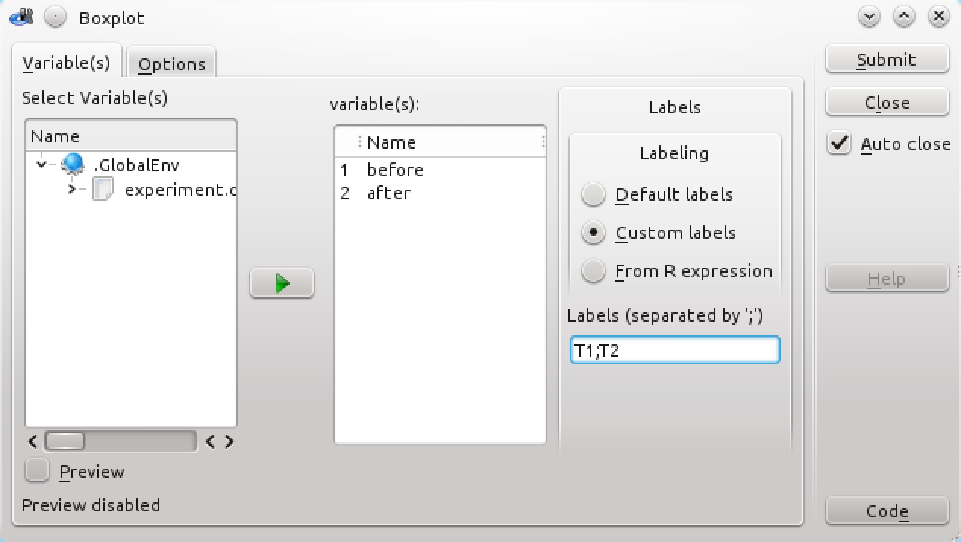
\includegraphics[width=15.5cm]{../figures/boxplot1.png}
 \caption{Boxplot dialog.}
 \label{fig:boxplot1}
\end{figure}

Checking the ``Preview'' box will open a graphics window, show the plot as
it is configured and update the window on changes in real time. From
that window it can be exported directly to several data formats as
well (Figure~\ref{fig:boxplot2}).

\begin{figure}[htp]
 \centering
 \includegraphics[width=15.5cm]{../figures/boxplot2.png}
 \caption{Plotted data and plot export dialog.}
 \label{fig:boxplot2}
\end{figure}

% !TEX root = RKWard_paper.tex
\section[Extending RKWard -- an example of creating a plugin]{Extending \pkg{RKWard} -- an example of creating a plugin}
\label{sec:example_plugin}
As discussed in Section~\ref{sec:technical_plugins}, plugins in \pkg{RKWard} are
defined by four separate files (Figure~\ref{fig:plugin_structure}). To give an impression of the technique,
this section shows (portions of) the relevant files for a plugin that provides
a simple dialog for a t-test. For brevity, the help-file is omitted.

\subsection{Defining the menu hierarchy}
\label{sec:defining_menu_hierarchy}
A so called ``.pluginmap'' file declares each plugin, and, if appropriate, defines where it should
be placed in the menu hierarchy. Usually each .pluginmap file declares many plugins. In this example
we only show one, namely, a two variable t-test (see Figure~\ref{fig:ttest-gui-example}). 
The pluginmap (\code{<!DOCTYPE rkpluginmap>}) gives a unique identifier (``id''), the location of the
GUI description (``file"), and the window title (``label''). The menu layout is defined in a hierarchical
structure by nesting \code{<menu>} elements to form toplevel menus and submenus. Menus with the same ``id''
are merged across .pluginmap files. Moreover, the position within the menu can be explicitly defined (attribute ``index'').
This might be required if the menu entries are to be ordered non-alphabetically.

\begin{footnotesize}
\begin{Code}
<!DOCTYPE rkpluginmap>
<document base_prefix="" namespace="rkward">
  <components>
    <component type="standard" id="t_test_two_vars"
          file="demo_t_test_two_vars.xml" label="Two Variable t-test" />
  </components>
  <hierarchy>
    <menu id="analysis" label="Analysis" index="4">
      <menu id="means" label="Means" index="4">
        <menu id="ttests" label="t-Tests">
          <entry component="t_test_two_vars" />
        </menu>
      </menu>
    </menu>
  </hierarchy>
</document>
\end{Code}
\end{footnotesize}


\begin{figure}[t!]
 \centering
 \includegraphics{../figures/ttest-gui-example.png}
 \caption{Generated menu structure as defined by the plugin map.}
 \label{fig:ttest-gui-example}
\end{figure}


\subsection {Defining the dialog GUI}
\label{sec:defining_dialog_ui}
The main XML file of each plugin defines the layout and behavior of the GUI, and references the
\proglang{ECMAScript} file that is used for generating \proglang{R} code from GUI settings and the help file (not included in this paper).

GUI logic can be defined directly in the XML file (the \code{<logic>} element).
In this example, the ``Assume equal variances'' checkbox is only enabled for paired sample tests.
Optionally, GUI behavior can also be scripted in \proglang{ECMAScript}.

The XML file defines the t-test plugin (\code{<!DOCTYPE rkplugin>}) to be organized in two tabs (Figure~\ref{fig:t_test}A).
On the first tab, two variables can be selected (\code{<varslot .../>}). These are set to be ``required'', i.\,e.,
the ``Submit'' button will remain disabled until the user has made a valid selection for both. The second tab includes some
additional settings like the confidence level (default 0.95).

\begin{footnotesize}
\begin{Code}
<!DOCTYPE rkplugin>
<document>
  <code file="demo_t_test_two_vars.js"/>
  <help file="demo_t_test_two_vars.rkh"/>

  <logic>
    <connect client="varequal.enabled" governor="paired.not"/>
  </logic>

  <dialog label="Two Variable t-Test">
    <tabbook>
      <tab label="Basic settings" id="tab_variables">
        <row id="basic_settings_row">
          <varselector id="vars"/>
          <column>
            <varslot type="numeric" id="x" source="vars" required="true"
              label="compare"/>                                                             
            <varslot type="numeric" id="y" source="vars" required="true"
              label="against"/>
            <radio id="hypothesis" label="using test hypothesis">
              <option value="two.sided" label="Two-sided"/>
              <option value="greater" label="First is greater"/>
              <option value="less" label="Second is greater"/>
            </radio>
            <checkbox id="paired" label="Paired sample" value="1" value_unchecked="0" />
          </column>
        </row>
      </tab>
      <tab label="Options" id="tab_options">
        <checkbox id="varequal" label="assume equal variances" value="1"
          value_unchecked="0"/>
        <frame label="Confidence Interval" id="confint_frame">
          <spinbox type="real" id="conflevel" label="confidence level" min="0" max="1"
            initial="0.95"/>
          <checkbox id="confint" label="print confidence interval" value="1"
            checked="true"/>
        </frame>
        <stretch/>
      </tab>
    </tabbook>
  </dialog>
</document>
\end{Code}
\end{footnotesize}

\subsection[Generating R code from GUI settings]{Generating \proglang{R} code from GUI settings}
\label{sec:generating_r_code_from_ui_settings}
A simple \proglang{ECMAScript} script is used to generate \proglang{R} code from GUI settings (using \code{echo()} commands)\footnote{
  See Figure~\ref{fig:t_test}A) for code generated in this example.
}. Generated code for each plugin is divided into three sections: ``Preprocess'', ``Calculate'', and ``Printout'', although each
may be empty.

\begin{footnotesize}
\begin{Code}
var x;
var y;
var varequal;
var paired;

function preprocess () {
  x = getValue ("x");
  y = getValue ("y");

  echo ('names <- rk.get.description (' + x + ", " + y + ')\n');
}

function calculate () {
  varequal = getValue ("varequal");
  paired = getValue ("paired");

  var conflevel = getValue ("conflevel");
  var hypothesis = getValue ("hypothesis");

  var options = ", alternative=\"" + hypothesis + "\"";
  if (paired) options += ", paired=TRUE";
  if ((!paired) && varequal) options += ", var.equal=TRUE";
  if (conflevel != "0.95") options += ", conf.level=" + conflevel;

  echo ('result <- t.test (' + x + ", " + y + options + ')\n');
}

function printout () {
  echo ('rk.header (result\$method, \n');
  echo ('  parameters=list ("Comparing", paste (names[1], "against", names[2]),\n');
  echo ('  "H1", rk.describe.alternative (result)');
  if (!paired) {
    echo (',\n');
    echo ('  "Equal variances", "');
    if (!varequal) echo ("not");
    echo (' assumed"');
  }
  echo ('))\n');
  echo ('\n');
  echo ('rk.results (list (\n');
  echo ('  \'Variable Name\'=names,\n');
  echo ('  \'estimated mean\'=result\$estimate,\n');
  echo ('  \'degrees of freedom\'=result\$parameter,\n');
  echo ('  t=result\$statistic,\n');
  echo ('  p=result\$p.value');
  if (getValue ("confint")) {
    echo (',\n');
    echo ('  \'confidence interval percent\'=(100 * attr(result\$conf.int, "conf.level")),\n');
    echo ('  \'confidence interval of difference\'=result\$conf.int ');
  }
  echo ('))\n');
}
\end{Code}
\end{footnotesize}


\bibliography{sources}
\end{document}
